\prefacesection{Business Understanding}

\section*{Business Understanding}
This dataset provides data on subjects with and without meningitis. It contains information such as age, gender, location, sum of health problems such as headaches, fevers and seizures. Additionally, is provides an attribute that indicate if the subject does or doesn't have meningitis, with a negative or positive value. 

\section*{Business Objective}

\begin{itemize}
	\item  Predict if someone is at risk of getting meningitis.
\end{itemize}

\section*{Data Mining objective}
\begin{itemize}
	\item The main objective is to create a model to predict the risk of a person getting meningitis 
	\item This model will use the attributes provided in the dataset such as age, gender, seizure history etc to assess the prediction accuracy.
	\item The model shall test multiple data mining algorithms to obtain a prediction.
\end{itemize}



\prefacesection{Data Understanding}

%- Describe the attributes in the dataset in terms of quality,
%information content, and usefulness
%- EDA Techniques
%- 3 charts

\section*{Describing Data}
In this section the allocated dataset is explained in terms of informational content, data quality and usability. The data set itself consists of attributes in relation to meningitis, a neuroligical infectious disease that can cause brain inflammation due to bacteria or viruses infecting that brain. As seen in tables below, the attributes have been segregated from numeric and categorical data. The numeric data given a description and a data type. Additionally, the mean, minimum, maximum and standard deviation values are given. Please refer to table \ref{table: numeric1} for information of the numeric data.


 \begin{longtable}{|c|>{\raggedright\arraybackslash}p{3cm}|c|c|c|c|c|}
	\hline
	\multicolumn{7}{| c |}{Numeric Attributes}\\
	\hline
	\textbf{Name} & \textbf{Description} & \textbf{Data type} & \textbf{Mean} & \textbf{Min} & \textbf{Max} & \textbf{SD}\\
	\hline
		AGE & List the age of each person & Numeric & 37.6285 & 10.0 & 84.0 & 15.3853\\
	\hline
		COLD & Number of days since last cold & Numeric & 2.6642 & 0.0 & 35.0 & 4.8273\\
	\hline
		HEADACHE & Days since last headache & Numeric & 7.1857 & 0.0 & 63.0 & 9.1278\\
	\hline
		FEVER & Days since last fevers&Numeric & 6.3428 & 0.0 & 63.0 & 8.0294\\
	\hline
		NAUSEA & Start of nausea & Numeric & 2.4857 & 0.0 & 32.0 & 4.5856\\
	\hline
		LOC & When loss of consciousness occurs &Numeric & 0.7428 & 0.0 & 26.0 & 2.6481\\
 	\hline
		SEIZURE & When convulsions are observed & Numeric & 0.1857 & 0.0 & 6.0 & 0.8780\\
	\hline
		BT & Body temperature & Numeric & 37.625 & 35.5 & 40.2 & 1.3041\\
	\hline
		STIFF & Neck stiffness & Numeric & 1.9571 & 0.0 & 5.0 & 1.4033\\
	\hline	
		KERNIG & Kernig sign & Numeric & 0.2142 & 0.0 & 1.0 & 0.4117\\
	\hline	
		LASEGUE & Lasegue sign & Numeric & 0.0785 & 0.0 & 1.0 & 0.2700\\
	\hline	
		GCS & Glasgow coma scale & Numeric & 14.7071 & 9.0 & 15.0 & 1.1536\\
	\hline
		WBC & White blood cell count  & Numeric & 8743.42 & 1070 & 90009 & 7795.80\\
	\hline
		CRP &  C-Reactive protein  & Numeric & 1.6878 & 0.0 & 31.0 & 4.1317\\
	\hline
		ESR & Blood sedimentation test  & Numeric & 5.9285 & 0.0 & 60.0 & 11.880\\
	\hline
		CSF\_CELL & Cell Count in Cerebulospinal Fluid & Numeric & 1505.4 & 0.0 & 63350 & 5708.83\\
	\hline
		Cell\_Poly & Polynuclear cell in CSF  & Numeric & 1025.85 & 0.0 & 61520 & 5402.38\\% \usepackage{array} is required
	\hline
		Cell\_Mono & Mononuclear cell in CSF  & Numeric & 465.08 & 0.0 & 7840 & 816.98\\
	\hline
		CSF\_PRO & Protein in CSF & Numeric & 99.414 & 0.0 & 474.0 & 96.307\\
	\hline
		CSF\_GLU & Glucose in CSF  & Numeric &  56.578& 0.0 & 520 & 44.3412\\
	\hline
		CSF\_CELL3 &  Cell Count CSF 3 days after the treatment & Numeric & 385.18 & 8 & 4860 & 1038.37\\
	\hline
		CSF\_CELL7 & Cell Count of CSF 7 days after treatment& Numeric & 205.61 & 0.0 & 7840 & 816.98\\
	\hline	
	\caption{Numeric Attribute Description.\label{long}}
	\label{table: numeric1}
\end{longtable}

The categorical dataset is given a description to the attribute labels and given a data type. Most of the attributes consist of only 2 values, but does of whom that are multivalued are displayed with the highest and lowest values in the table. See table \ref{table: nominal1} for further insight to the dataset.

 \begin{longtable}{|c|>{\raggedright\arraybackslash}p{4cm}|c|c|c|}
	\hline
	\multicolumn{5}{| c |}{Categorical Attributes}\\
	\hline
	\textbf{Name} & \textbf{Description} &\textbf{Data type} &\textbf{Value 1} &\textbf{Value 2}\\
	\hline
		SEX & Gender of people & Nominal & M (82) & F (58) \\	
	\hline
		Diag2 & Diagnoses & Nominal & VIRUS (98) & BACTERIA (42) \\	
	\hline	
		ONSET & Inception & Nominal &  CHRONIC (1) & ACUTE (130)  \\	
	\hline	
	 	LOC\_DAT & Loss of consciousness& Nominal & - (98) & + (42) \\	
	\hline	
		FOCAL & Focal Sign& Nominal & - (105) & + (35) \\	
	\hline	
		CT\_FIND &  CT findings & Nominal & normal (101) & abnormal (39) \\	
	\hline	
		EEG\_WAVE& Electroencephalography Wave Findings  & Nominal & abnormal (117) & normal (23) \\	
	\hline	
		EEG\_FOCUS & Focal sign in EEG & Nominal & -(104) & +(36) \\	
	\hline	
		CULT\_FIND & If bacteria or virus found & Nominal & F (107) & T(33) \\	
	\hline	
		CULTURE & Name of bacteria/virus found & Nominal & Tb (1) & - (107) \\	
	\hline	
		THERAPY2 & Therapy & Nominal & PIPC+CTX (1) & no\_therapy (58) \\	
	\hline	
		C\_COURSE & Clinical course at discharge & Nominal & negative (117) & paralysis (1) \\	
	\hline	
		COURSE(Grouped) & Grouped attribute of C\_COURSE & Nominal & n (117) & p (23) \\	
	\hline	
		RISK(Grouped) & Class label - at risk  & Nominal & n (121) & p (19) \\	
	\hline		
	\caption{Categorical Attribute Description.\label{long}}
	\label{table: nominal1}		
\end{longtable}

The data above could be divided into a number of sections. Attributes such as AGE and SEX can be categorized as \textit{personal information}. COLD, HEADACHE, NAUSEA LOC etc. can be described as \textit{subject history} as they provide some information on the commencement of the symptoms. BT, STIFF, KERNIG, GCS can be assigned to a category of \textit{physical examination} as they attribute values obtained during investigation. Further more, \textit{laboratory investigation} used to describe the attributes such as WBC, EEG\_WAVE, CULT\_FIND, ESR etc. These are values collected during further investigate of the bodily anomalies. Lastly, \textit{postliminary treatment} if used to describe THERAPY2, CSF\_CELL3 and CSF\_CELL7 as they are attributes describing values after a subject has been treated for meningitis. 
The dimensionality of the dataset is a total of 36 attributes and there are 141 instances.
\section*{Data Exploration}
The following section will utilize the Exploratory Data Analysis (EDA) techniques to further analyze the data. This will give insight on how to improve the quality of the data and reduce dimensionality among the dataset. It shall also provide a number of charts to visually represent the data in regards to attributes that may prove to be predictive, show indication of correlations, and data with low variability. \\
As seen in Figure\ref{symp} a histogram is used to plot out the main symptoms of meningitis. This consists of the attributes COLD, HEADACHE, FEVER, NAUSEA. The values are attributed to the amount of days since these sensations have been felt. Therefore they are applicable to the mining objectives as they appear to be very predictive.
\begin{figure}[ht]
	\begin{center}
		\advance\leftskip-3cm
		\advance\rightskip-3cm
		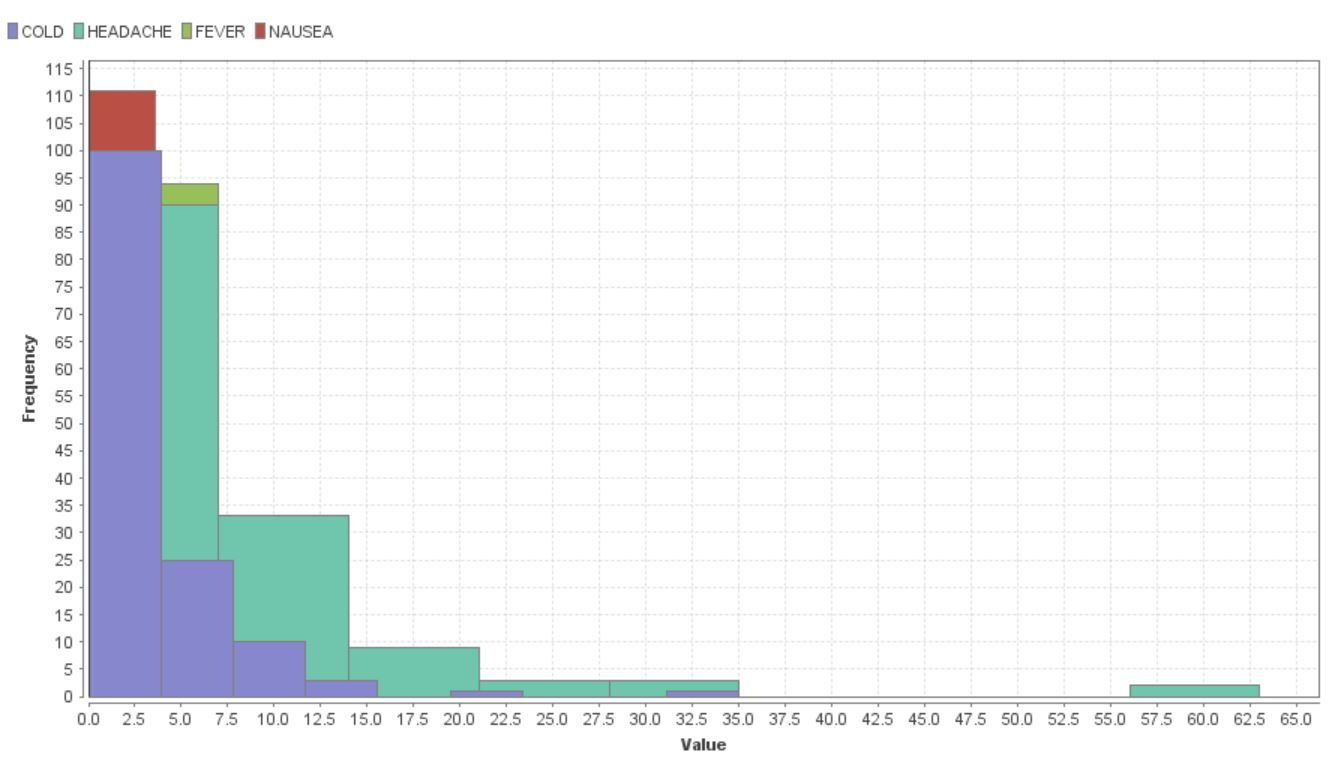
\includegraphics[keepaspectratio=true,scale=0.6]{__resources/symptoms.jpg}
		\caption{Main symptoms for meningitis}
		\label{symp}
	\end{center}
\end{figure}
\newpage
Furthermore, a high correlation between the attributes ONSET and CSF\_CELL3 can be seen in Figure \ref{onset}. Due to this high correlation one of these attributes can be removed from the dataset as they are redundant. Furthermore. They are scarce in values so they may not prove beneficial to the mining objectives.
\begin{figure}[ht]
	\begin{center}
		\advance\leftskip-3cm
		\advance\rightskip-3cm
		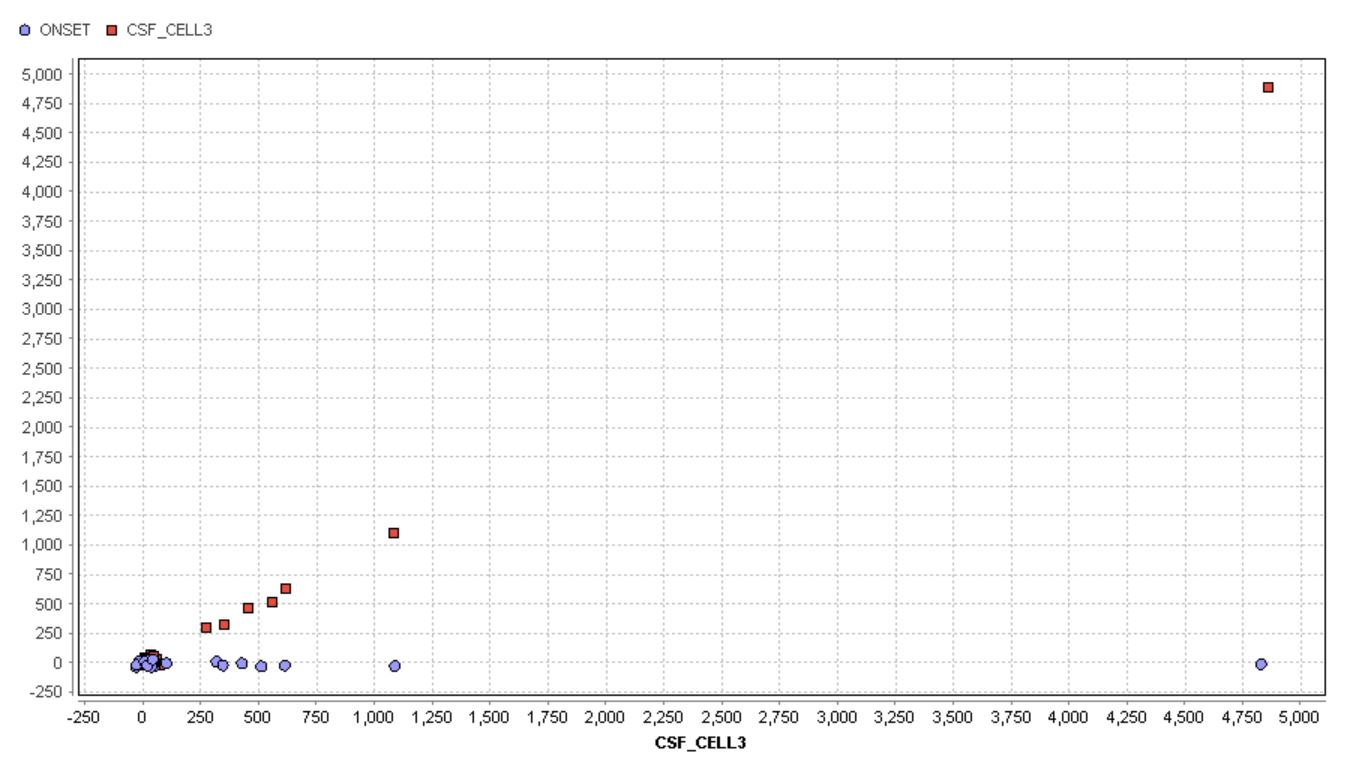
\includegraphics[keepaspectratio=true,scale=0.6]{__resources/onset_csf_cell3.jpg}
		\caption{Scatter plot for ONSET and CSF\_CELL3}
		\label{onset}
	\end{center}
\end{figure}

\newpage

The following histogram displays the values for positive (P) and negative (N) in the class label RISK(Grouped).This unbalance in inequitable group of values may prove to cause some difficulties as it may falsely predict everyone to be negative(n) for risk of having meningitis.
See Figure \ref{risk} below.
\begin{figure}[ht]
	\begin{center}
		\advance\leftskip-3cm
		\advance\rightskip-3cm
		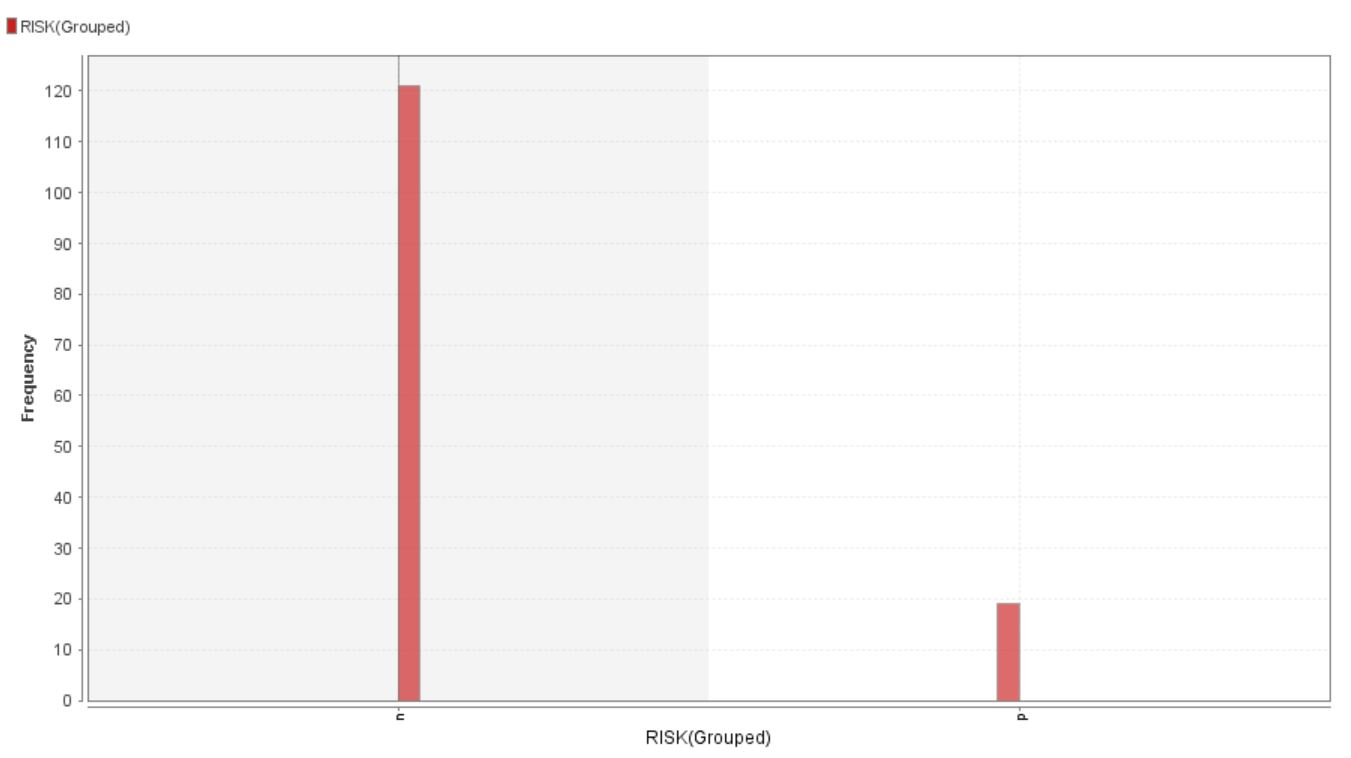
\includegraphics[keepaspectratio=true,scale=0.6]{__resources/risk.jpg}
		\caption{Histogram for class label RISK(Grouped)}
		\label{risk}
	\end{center}
\end{figure}

\newpage
Figure \ref{box}  shows a box plot of CSF\_PRO the distribution of data. Although these values may prove beneficial in distinguishing between at risk and not at risk for meningitis, there are some outlier values seen which can skew the data.  

\begin{figure}[ht]
	\begin{center}
		\advance\leftskip-3cm
		\advance\rightskip-3cm
		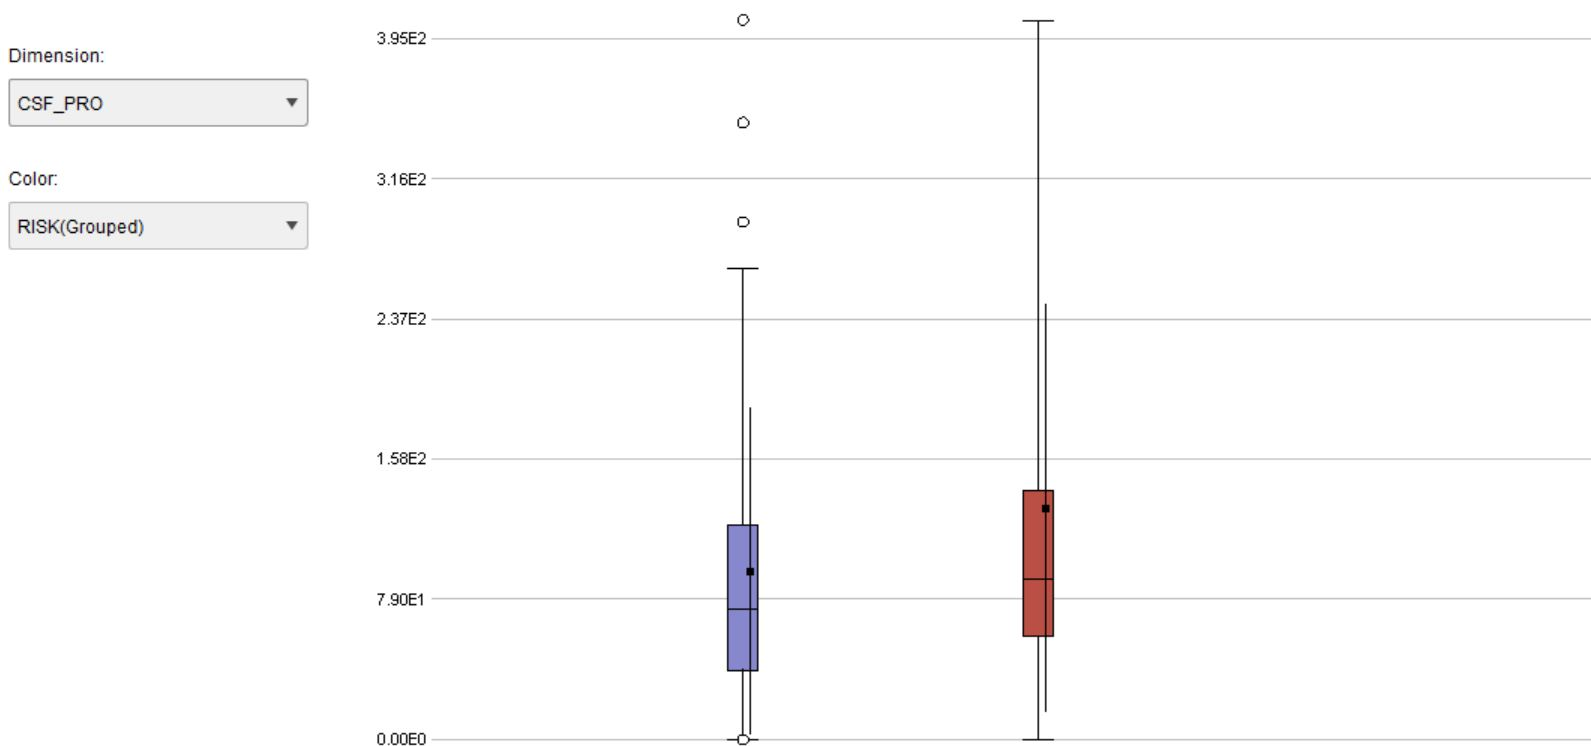
\includegraphics[keepaspectratio=true,scale=0.6]{__resources/boxplot.jpg}
		\caption{Protein in Cerebulospinal Fluid}
		\label{box}
	\end{center}
\end{figure}

%WBC count would be good to use as the variance of data isn't too big
%-- box plot this


%CSF_CELL3 correlates with ONSET so it can go
\newpage

\section*{Verifying Data Quality}

\textbf{Missing Values}\\
Some missing values can be found in this data set. For example, row 122 contains no values at all. Additionally, CSF\_CELL3 has a lot of missing data. There are a total of 119 out of the 141 instances of CSF\_CELL3 that a missing values. This means that there are only 22 rows in the entire dataset that do not contain any missing data. \\
\textbf{Noise, Bias and Outlier Values}\\
Many outlier values can be seen. For instance, the FEVER attribute has a mean value of 6.343. But this value may be skewed as there is a high outlier value, 63, at row 8. Furthermore, the value 90009.0 in the white blood cell count (WBC). This may be an erroneous value as the next highest value in the column is only 19500. This outlier value may disrupt the accuracy of prediction in the model.\\
\textbf{Sufficient Attributes}\\
There are some redundant attributes found in the dataset. One example of this is the SEIZURE attribute. There are only 8 individual and 4 distinct instances therefore it would be insufficient for representation of a class. Secondly, the CULT\_FIND and CULTURE represent the same data. CULTURE would be more sufficient for prediction as it contain more varied values of bacteria/viruses found such as influenza, tb, herpes, strepto etc. rather than the true or false values of CULT\_FIND. Therefore CULT\_FIND can be removed from the dataset.

%Row 122 has no values
%CSF_CELL3 has a lot of missing values
%CSF_CELL7 has a lot of 0 
%SEIZURE only has 8 individual instances which isn't
% sufficient to represent the class
%Insufficient class label distribution of data


\prefacesection{Data Preparation}
Firstly, the model was tested using a decision tree without any data preprocessing. Firstly, the attribute RISK(Grouped) was assigned as the class label. As many rows contain missing values, a filter was applied to ignore this row of data using the \textit{no\_missing\_attribute} condition class. The split validation operator was then used for splitting the dataset in a training and testing data set with a split ratio of 0.7. Initially, linear sampling was used for testing the model. This gave an accuracy result of 57.14\%. Shuffled sampling was used, which randomly selects 70\% of the rows in the dataset as training data.This returned a result of 85.71\% percent. Lastly, stratified sampling was used to select 70\% of the rows from each class and this gave a result of 83.33\%. Secondly, the k-Nearest Neighbor (k-NN) algorithm was used. Linear sampling and shuffled sampling with k-NN both provided an accuracy of 57.14\% and stratified sampling gave an accuracy of 66.67\%.
\\Although these accuracies are relatively high, they are only trained on 22 rows of values. This provides a false accuracy as the dataset is not large enough. Therefore, further preprocessing measures are needed to give a fairer accuracy result.



%  three data preparation techniques to use
%Justify the choices made: Discuss why your chosen techniques are appropriate/required for this data set and mining objective. 
% Document the improvements,
\subsection*{Select Data}
There is not a high number rows need to be removed from the dataset as there should be at least 20 times more rows that columns in a dataset. However, some of the rows or columns may be transformed due to missing values, which shall be addressed in the following section.
\subsection*{Clean Data}
Due to missing data in a number of cells in the dataset a number of transformational steps must be taken to ensure an increase in the overall accuracy of the final model. As row 122 is the only row in the dataset that has a large amount of missing data, it shall be removed from the dataset as it makes up less then 5\% of the number of rows, therefore it will not significantly affect the final result. This was implemented using the \textit{Filter Example Range}, which was used to filter out row 122 from the dataset. Using stratified sampling with a decision tree, this produced an accuracy of 73.81\%. Please refer to Figure \ref{122}

\begin{figure}[ht]
	\begin{center}
		\advance\leftskip-3cm
		\advance\rightskip-3cm
		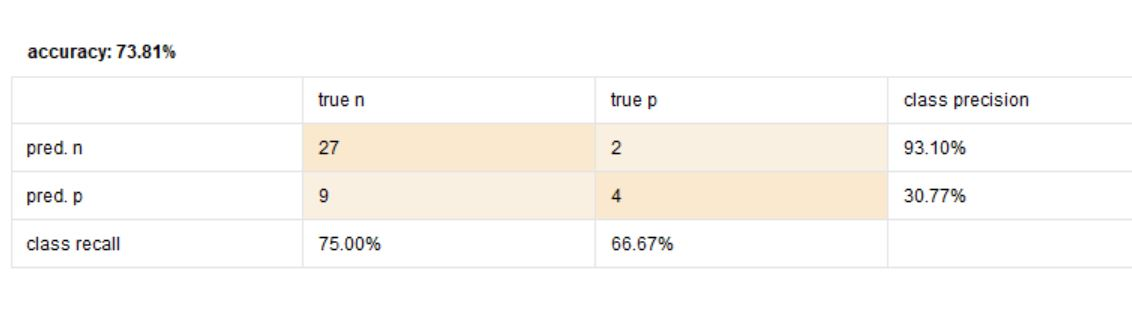
\includegraphics[keepaspectratio=true,scale=0.6]{__resources/122Filter.jpg}
		\caption{Stratified Sampling Using a Decision Tree}
		\label{122}
	\end{center}
\end{figure}

The attribute CSF\_CELL3 lacks a lot of values. There are a total of 119 rows out of 141 that contain no value at all which means there is an  84.4\% value absence. This column shall be removed as it is missing more than 40\% of it's values. This is applied using the \textit{Select Attributes} Filter and exclude CSF\_CELL3 from the dataset. There are other attribute that should also be removed. For example, attributes such as LASUGUE, and GCS should be removed because to provide too little variance in values to the dataset. Following the application of these steps, the accuracy of the model has risen from 73.81\% to 78.57\%, as seen in Figure \ref{filtering}. \\ 
\begin{figure}[ht]
	\begin{center}
		\advance\leftskip-3cm
		\advance\rightskip-3cm
		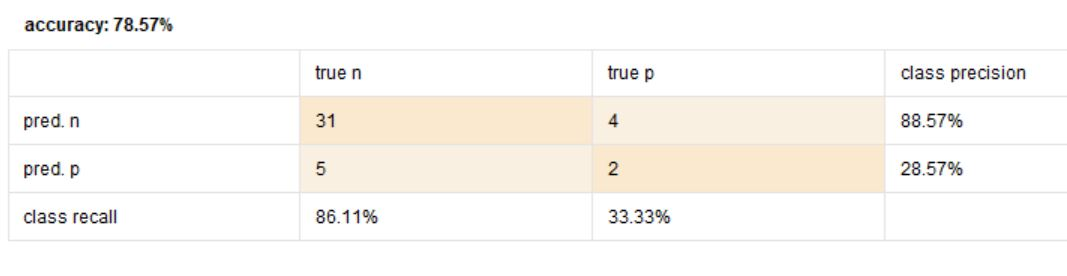
\includegraphics[keepaspectratio=true,scale=0.6]{__resources/gcsfilter.jpg}
		\caption{Results After Filtering Useless Attributes}
		\label{filtering}
	\end{center}
\end{figure}
\\\\\\\\\\\\
More ever, WBC possibly has a very high value outlier value of 90009. To accommodate for this \textit{outlier detection} is used to to filter out this value. However, this did not increase the accuracy significantly so it was not kept for further testing. 
In order to reduce the dimensionality of the data, correlating attributes were removed. This was done by using the \textit{Remove Correlated Attributes} operator. A threshold of 95\% was used to filter out the highly correlated columns. In turn, this increased the accuracy by of the model from 78.57\% to 85.71\%. Although this accuracy is relatively high, the class recall and class precision for \textbf{true p} was at a 50/50 split. Therefore it would not accurately predict positive risk subjects. Construction of new data will be used to address this problem, which will be touched upon in the next section.

\subsection*{Construct Data}
Seeing as the Meningitis Dataset is relatively small, only having 141 rows, it is not sufficient for modeling. There should be atleast 20 times more rows in a dataset than attributes. Proceeding the initial preprocessing steps, there are a total of 32 attributes in the dataset. Therefore, there should be at least 640 rows. To address this problem, a number of sampling steps were taken. Initially, progressive sampling was used to increase the size of the data. This returned an accuracy of 90.48\%, also increasing the class precision from 50\% to 75\%. The second approach taken was stratified sampling, which proves beneficial when the number of possible classes are known. No increase in performance was seen in this approach so the next sampling technique was taken. Kennard-Stone sampling then tested. Kennard-Stone sampling selects the two rows  that are the furthest from one another and then adds other rows are added by adding new rows thats are furthers from objects currently being sampled. Due to the nature of the Kennard-Stone algorithm, only numeric values can be handled. The \textit{Nominal to Numberic} operator was then used to handle this in regard to nominal values. This approach gave an accuracy of 90.48\% and a class recall of \textbf{true p} of 33.33\%. \\
The last approach taken was applying a bootstrapping technique to the data, which involves creating new data from the preexisting data. Using the \textit{sample\_bootstrapping} operator, an absolute value was initially created with 200 samples to start off with. This produced an accuracy of 95\%. 300 samples were then tested, which gave back an accuracy of 93.33\%. These 100 sample interval steps were taken all the way to 600 samples. Which then gave an accuracy of 98.33\%. Although this accuracy may appear high, it should be acknowledged that when using bootstrap, this accuracy is an over estimation.\\
Due to class imbalance and the under representation of class of people who are positive of risk of meningitis, Sampling is needed to equalize the classes out. This is done by filtering class \textbf{p} and bootstrapping new data to the dataset. Considering the dataset is relatively small, bootstrapping is applied to both classes in order to have a sufficient amount of examples. In total there is a 50/50 split of class labels with a total of 640 examples (20 times the amount of attributes). Please see the Figure \ref{balance} for chart of the class label. At this stage, there is a 97.4\% accuracy rate.

\begin{figure}[ht]
	\begin{center}
		\advance\leftskip-3cm
		\advance\rightskip-3cm
		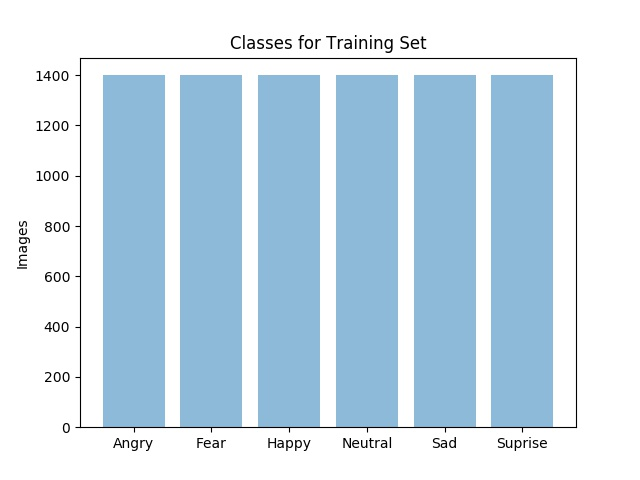
\includegraphics[keepaspectratio=true,scale=0.6]{__resources/balance.jpg}
		\caption{Balanced Classes for RISK(Grouped)}
		\label{balance}
	\end{center}
\end{figure}


\prefacesection{Modeling}
\section*{Modeling technique}
For this mining objective, algorithms that are good for classification rather than prediction is necessary as the the dataset contains nominal values. Therefore, some of the most suitable algorithms for this problem are Decision Trees as output can be easily understood, Artificial Neural Networks as they can be used for prediction or classification.
\section*{Test Design}
Cross validation will be utilized for creating the test and training data. Where \textit{k=5} and using a shuffled sampling type.Using this approach allows for the entire dataset to be used for testing and training. 
For evaluation on the model, the accuracy will highlight for the different parameters being used in the model.

\section*{Build and Assess the Model}
\subsection*{Decision Tree}
The Decision tree model was first implemented using the preprocessing steps stated in the previous section. K-fold cross validation was then used to create the training and testing data. On the decision tree operator, pruning and prepruning is applied to reduce the complexity of the classifier. Firstly, 5 fold were used, working up until a maximal accuracy value was found. Please see the table below for accuracy results.

\begin{longtable}{|>{\raggedright\arraybackslash}p{2cm}|c|}

	\hline
	\textbf{Number of Folds} & \textbf{Accuracy}\\
	\hline 
	5 & 97.19\% \\ 
	\hline 
	6 & 97.34\% \\ 
	\hline 
	7 &  97.66\%\\ 
	\hline 
	8 & 97.66\% \\ 
	\hline 
	9 &  97.50\%\\ 
	\hline 
	10& 97.81\% \\ 
	\hline 
	11& 97.82\% \\ 
	\hline 
	12&   97.81\%\\ 
	\hline 
	13&  97.50\%\\ 
	\hline 
	14&  97.65\%\\ 
	\hline 
	\caption{Cross Validation - Decision Tree\label{long}}
	\label{table: folds}		
\end{longtable}

As seen in the Table \ref{table: folds} the optimal number of folds is 11 for the highest accuracy at a total of 97.82\%. The decision tree is properly fitted, as there isn't too little or too many branches in the model. See Figure \ref{tree} for a diagram of the decision tree

\begin{figure}[ht]
	\begin{center}
		\advance\leftskip-3cm
		\advance\rightskip-3cm
		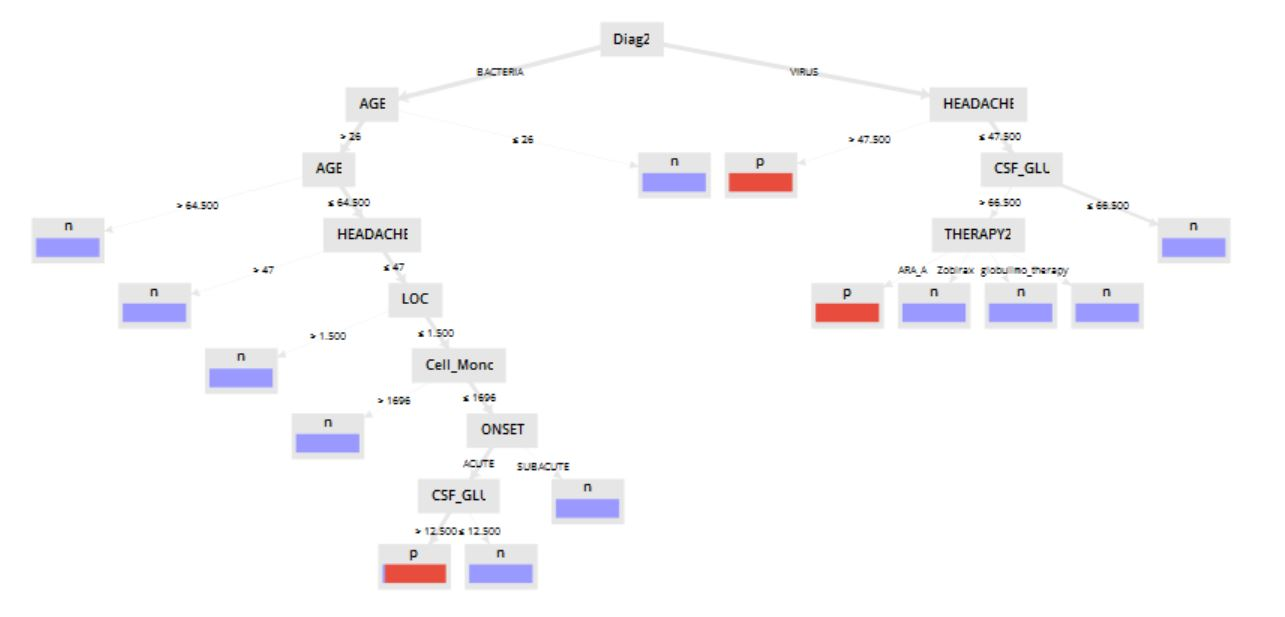
\includegraphics[keepaspectratio=true,scale=0.6]{__resources/tree.jpg}
		\caption{Decision Tree }
		\label{tree}
	\end{center}
\end{figure}

\newpage

\subsection*{Artificial Neural Network}
The artificial neural was first implemented using the preprocessing steps stated in the previous section. For training and testing data, cross validation was utilized with 11 folds as it proved to be the optimal parameter for validation. The \textit{Deep learning} operator was used as back-propagation is good for training model for higher accuracy. The model used ReLU as it's activation function. The number of epochs are then specified, incremental steps in the number of epochs were tested to find the best accuracy. Five runs were conducted for each interval of epochs tests, each accuracy score was recorded and an average percentage given. \\

\begin{longtable}{|>{\raggedright\arraybackslash}p{3cm}|c|}
	
	\hline
	\textbf{Number of Epochs} & \textbf{Average Accuracy}\\
	\hline 
	5 & 97.81 + 97.66 + 98.44 + 97.81 + 97.65 /5 = \textbf{97.87\%} \\ 
	\hline 
	10 & 98.90 + 98.90 + 98.91 + 98.29 + 98.91 /5 = \textbf{98.78\%} \\ 
	\hline 
	15 &  99.69 + 99.37 + 99.37 +  99.37 + 99.06 /5 =  \textbf{99.37\%}\\ 
	\hline 
	20 & 99.84 + 99.37 + 99.53 + 99.22 + 99.22 /5 = \textbf{99.43\% }\\ 
	\hline 
	25 & 98.44 + 98.43 + 99.69 + 99.07 + 99.53 /5 = \textbf{99.03\% }\\ 
	\hline 
	\textbf{Average Overall Accuracy} & \textbf{98.89\% }\\
	\hline
	\caption{Artificial Neural Network Test Results\label{long}}
	\label{table: ann}		
\end{longtable}

As seen in the table \ref{table: ann} above, the optimal amount of epoch for this dataset found was 20, giving the highest accuracy of 99.43\% and an overall average accuracy of 98.89\%. In terms of performance, this approach could be improved in terms of speed as neural networks are computationally expensive, therefore faster hardware would boost training time.

\prefacesection{Evaluation}
To conclude, the mining objective have been achieved. A model that can accurately predict if a person is at risk of meningitis was successfully implemented using the Meningitis Dataset. Two techniques were used, giving accuracy results of 97.82\% and 99.43\%. 

The models perform well given the limitations of the dataset, being it's small size, and quality issues. In terms of accuracy, Artificial Neural Networks out done the rest due to it's high results, but lacks in performance of speed due to it's slow computation time. Overall, the business and mining objectives have been met and the project has been completed successfully.

